\chapter{Evaluation}
\label{cha:evaluation}
In this chapter, we present a comprehensive evaluation of two models, namely Model 1 and Model 2, designed for web tracker detection.
Additionally, we assess the performance of our real-time web application. The evaluation aims to provide insights into the effectiveness,
accuracy, and practicality of the models and their application in detecting web trackers in real-time.

The evaluation process involves rigorous analysis of the models' performance using various metrics, including accuracy, precision,
recall, F1-score, and false positives/negatives. These metrics enable us to assess the models' ability to correctly classify web
requests as either tracker or non-tracker, thereby enhancing user privacy and security during web browsing.

Furthermore, we assess the real-time web application that integrates these models. The application's performance is evaluated in
terms of its ability to detect web trackers in real-time. For that we conducted web crawls of the Tranco Top 1K visited websites
and evaluate the amount of requests performed. Additionally, we analyze the impact of the application on browsing performance.
\section{Models}
In this section, we look at the experimental setup and the training of the two models. The first model uses the feature vector of dimension [204, 1] 
which can be seen in Fig-\ref{fig:featModel1} and the second model uses the feature vector of dimension [233, 1]
which can be seen in Fig-\ref{fig:featModel2}. Moreover, we evaluate the training process of the models, the training results and look
at the limitations of this setup.

\subsection{Training}
We outline the training process for both Model 1 and Model 2.
We provide a detailed overview of the training methodology employed, emphasizing the techniques utilized to address
the class imbalance present in the dataset. The used dataset was generated from a web crawl of the Tranco Top 10K websites. 
However, the presence of web tracker in comparison to non tracker is significant lower when browsing the web. There are fewer trackers (256,273) than non-trackers (594,865) present in the dataset. This class imbalances can affect the
model's performance and bias its predictions towards the majority class.

To address the class imbalance, we utilized oversampling and undersampling techniques. Initially, we employed the \emph{RandomOverSampler},
which duplicates instances from the minority class (trackers) to equalize their representation with the majority class (non-trackers).
This technique enables the model to learn from a more balanced dataset and prevents it from being biased towards the majority class.

Subsequently, we utilized the \emph{RandomUnderSampler} to randomly select instances from the majority class, effectively reducing its
dominance in the training set. By undersampling the majority class, we further alleviate the class imbalance, ensuring that both
classes have a comparable number of instances during model training.

After generating a balanced training set, we constructed the model architecture using a sequential approach in TensorFlow.
The model architecture is described in Fig-\ref{fig:modelStructure}.
Furthermore, we compiled the model by selecting the mean squared
error (MSE) loss function and employed the RMSprop optimizer. The MSE loss function measures the discrepancy between the predicted
and actual labels, while the RMSprop optimizer adjusts the model's parameters to minimize this loss.

During the training phase, we utilized a training set that is comprised of the balanced samples (X\_train and y\_train) generated
through oversampling and undersampling. The model was trained using this dataset, specifying the batch size (512) and the number
of epochs (10). To assess the model's performance during training and prevent overfitting, we incorporated a validation set
(X\_test and y\_test) to monitor the model's progress and to detect any signs of under or overfitting.

Following the completion of the training process, we evaluated the trained model's performance using various metrics.
We calculated the test loss and test accuracy, which provide insights into the model's overall performance on the unseen
test data. These metrics enable us to gauge the model's ability to accurately classify web requests as either tracker
or non-tracker.

\subsection{Model 1}

Upon completion of
the training process, Model 1 exhibited promising performance on the test dataset. The evaluation metrics provide valuable insights
into its accuracy, precision, recall, F1-score, and other important measures.


\begin{figure}[ht!]  
  \centering
  \begin{subfigure}[b]{.47\textwidth}
      \centering
      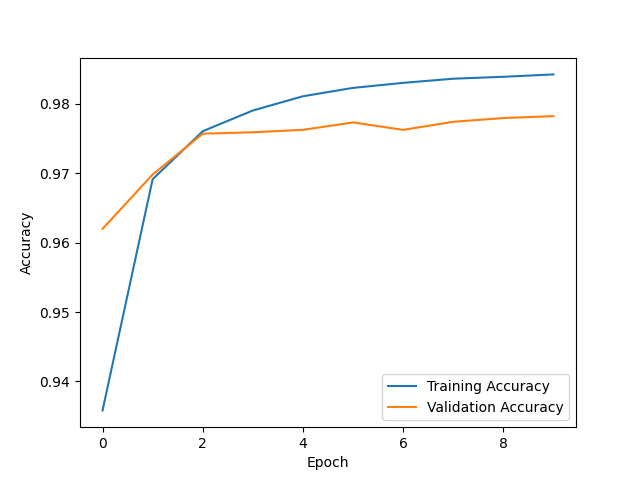
\includegraphics[width=\linewidth ]{images/M1_ACC_fin.png}
      \caption{This figure exhibits the accuracy of Model 1 in training process. The x-axis shows the training epoch and the y-axis 
      displays the accuracy. The blue graph shows the accuracy on the training data and the orange graph shows the accuracy on the test data.
    The plot shows that the model convergence and generalizes well with the underlying training data. }
      \label{fig:accM1}
  \end{subfigure}
  \hfill
  \begin{subfigure}[b]{.47\textwidth}
      \centering
      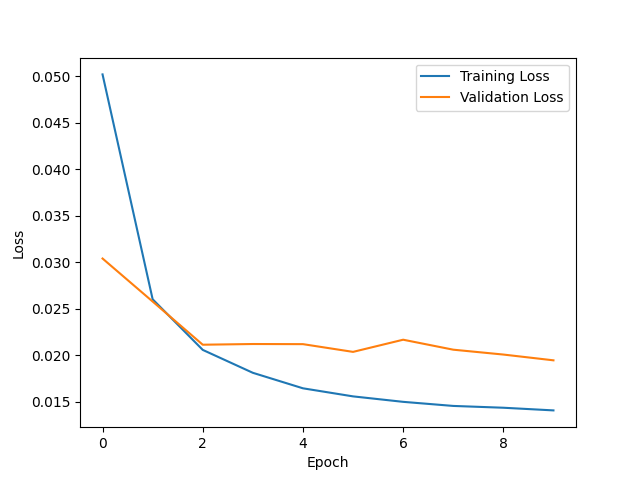
\includegraphics[width=\linewidth, keepaspectratio]{images/M1_Loss_Fin.png}
      \caption{This figure manifests the loss of Model 1 during the training process. The x-axis shows the training epoch whereas the y-axis shows
      the training loss. The blue graph explains the loss on the training data whereas the orange graph explains the loss on the test data. 
      This graphs additionally underlines that the model convergence and generalizes well.
    }
      \label{fig:lossM1}
  \end{subfigure}
  \label{}
  \caption{This figure unveils the loss and the accuracy of Model 1 regarding the training epoch. Both figures show a great convergence and generalization.}
\end{figure}
As shown in Fig-\ref{fig:lossM1}, the test loss obtained for Model 1 was \emph{0.019}, indicating the average dissimilarity between the 
predicted and actual labels. A lower test loss indicates better model performance, suggesting that Model 1 achieved good alignment
with the true labels in the test dataset. Furthermore, as shown in Fig-\ref{fig:accM1}, the test accuracy of Model 1 was determined
to be \emph{0.98}. This metric measures the proportion of correctly classified instances out of the total number of instances in
the test dataset. With a high accuracy score of \emph{98\%}, Model 1 demonstrates its proficiency in accurately classifying web
requests as either trackers or non-trackers.

\begin{table}[ht!]
  \begin{center}
    \begin{tabular}[c]{|l|l|l|l|l|}
      \hline
      \multicolumn{5}{|c|}{\textbf{Classification Report: Model 1}} \\
      \hline
      \textbf{} & \textbf{precision} & \textbf{recall} & \textbf{f1-score} & \textbf{support} \\
      \hline
      non-tracker & 0.98 & 0.99 & 0.98 & 195,982 \\
      \hline
      tracker & 0.97 & 0.96 & 0.96 & 84,894 \\
      \hline
      accuracy & & & 0.98 & 280,876 \\
      \hline
      macro avg & 0.98 & 0.97 & 0.97 & 280,876 \\
      \hline
      weighted avg & 0.98 & 0.98 & 0.98 & 280,876 \\
      
      \hline
    \end{tabular}
  \end{center}
  \caption{The table presents the classification report for Model 1, which was developed to detect trackers and non-trackers
  in web requests. The report provides detailed performance metrics, including precision, recall, and F1-score, for each class.
The table demonstrates the model's ability to accurately classify non-trackers and trackers, showcasing
its precision in correctly identifying instances of each class.}
  \label{tab:m1}
\end{table}

The classification report, which is shown in Tab-\ref{tab:m1}, provides an overview of the precision, recall, and F1-score for each class.
For non-trackers, Model 1 achieved a precision of 0.98. Precision represents the proportion of true non-trackers
out of all instances classified as non-trackers. Therefore, a precision of 0.98 indicates that Model 1 has a high precision
in correctly identifying non-trackers. Out of all instances classified as non-trackers, 98\% are indeed non-trackers.

Additionally, Model 1 achieved a recall of 0.99 for Class 0. Recall, also known as sensitivity or true positive rate, measures
the proportion of true non-trackers correctly identified by the model out of all actual non-tracker instances. A recall of 0.99
indicates that Model 1 has a high recall in capturing the majority of non-tracker instances. It correctly identifies 99\% of the
actual non-trackers present in the dataset.

The F1-score for non-trackers is calculated as 0.98. The F1-score is the harmonic mean of precision and recall, providing a balanced
measure of a model's performance. With an F1-score of 0.98, Model 1 demonstrates a high overall accuracy in correctly identifying
non-trackers.

Moving to trackers, Model 1 achieved a precision of 0.97. This precision value indicates that out of all instances
classified as trackers, 97\% are actually trackers. The model has a high precision in accurately identifying tracker instances.
The recall for Class 1 is 0.96, implying that Model 1 captures 96\% of the true tracker instances out of all actual tracker
instances in the dataset. The recall, in this case, represents the ability of the model to detect trackers effectively.

The F1-score for trackers is calculated as 0.96. This value accounts for both precision and recall and provides an overall
measure of the model's performance in identifying trackers. With an F1-score of 0.96, Model 1 demonstrates a strong ability
to accurately identify tracker instances, although with a slightly lower precision and recall compared to non-trackers.

Analyzing the classification report as a whole, we observe an overall accuracy of 0.98, indicating that Model 1 correctly
classifies 98\% of the instances in the test dataset. The macro average F1-score is 0.97, which considers the F1-score
for each class and provides a measure of the model's performance across classes, giving equal weight to both classes.
The weighted average F1-score is also 0.98, which considers the F1-score weighted by the support (the number of instances)
for each class. This demonstrates the overall effectiveness of Model 1 in detecting both trackers and non-trackers.

In conclusion, Model 1 shows high precision, recall, and F1-scores for both classes. It accurately identifies non-trackers
with a precision of 0.98 and a recall of 0.99, while also demonstrating the ability to identify trackers with a precision of 0.97
and a recall of 0.96. These results indicate the model's proficiency in distinguishing between tracker and non-tracker web requests.
The classification report, along with other evaluation metrics, reinforces the reliability and effectiveness of Model 1 in detecting
web trackers.

\subsection{Model 2}

Model 2, also demonstrates strong performance in detecting web trackers. The training process of Model 2 shows a great convergence 
and generalization, which is indicated in Fig-\ref{fig:lossaccM2}. The graphs are similar to the graphs of Model 1, but the accuracy
is slightly lower. The classification
report provides valuable insights into the precision, recall, and F1-scores for each class. For non-trackers, Model 2
achieved a precision of 0.99, indicating that it accurately identifies 99\% of the instances classified as non-trackers.
This high precision suggests a high level of confidence in correctly identifying non-trackers. 
Regarding recall, Model 2 achieved a recall of 0.98 for non-trackers. With that recall, Model 2 effectively captures 98\% of
the non-tracker instances present in the dataset, highlighting its ability to identify the majority of non-tracker web requests.
The F1-score for non-trackers is 0.98, which indicates that Model 2 achieves a balanced performance
in detecting non-trackers.

\begin{figure}[ht!]  
  \centering
  \begin{subfigure}[b]{.47\textwidth}
      \centering
      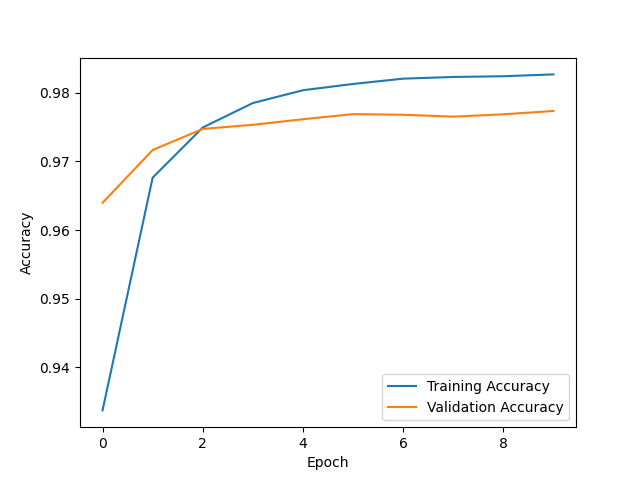
\includegraphics[width=\linewidth ]{images/Model2Acc.png}
      \caption{This figure illustrates the accuracy of the model in training process. The x-axis shows the training epoch and the y-axis 
      displays the accuracy. The blue graph shows the accuracy on the training data and the orange graph shows the accuracy on the test data.
    The plot demonstrates that the model convergence and generalizes well with the underlying training data.}
      \label{fig:accM2}
  \end{subfigure}
  \hfill
  \begin{subfigure}[b]{.47\textwidth}
      \centering
      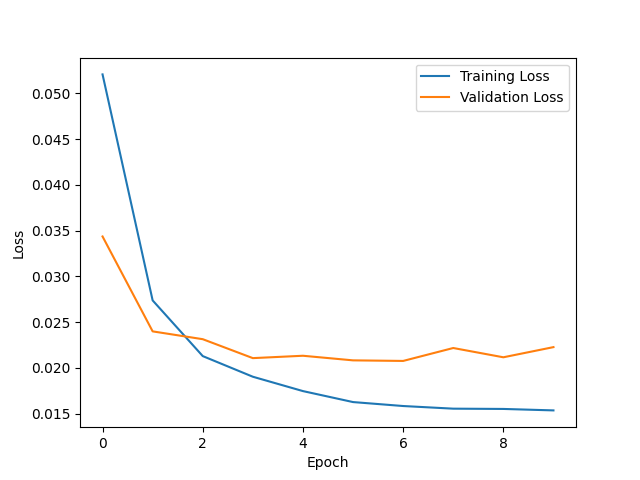
\includegraphics[width=\linewidth, keepaspectratio]{images/M2_Loss_Fin.png}
      \caption{This figure presents the loss of the model training process. The x-axis reveals the training epoch whereas the y-axis depicts
      the training loss. The blue graph explains the loss on the training data whereas the orange graph elaborates the loss on the test data. 
      This graphs additionally underlines that the model convergence and generalizes well.
    }
      \label{fig:lossM2}
  \end{subfigure}
  \caption{This figure shows the loss and the accuracy of Model 2 regarding the training epoch. Both figures show a great convergence and generalization.}
  \label{fig:lossaccM2}
\end{figure}
Moving to trackers, Model 2 achieved a precision of 0.95. This precision value indicates that out of all instances
classified as trackers, 95\% are indeed trackers. The model demonstrates a high precision in accurately identifying tracker instances.
Moreover, a recall of 0.97 was achieved, which suggests that Model 2 captures 97\% of the actual tracker instances
out of all tracker instances present in the dataset. The model exhibits a strong ability to detect trackers effectively.
Furthermore, for the class trackers Model 2 achieved an F1-score of 0.96, which demonstrates a solid ability to accurately
identify tracker instances, although with a slightly lower precision and recall compared to non-trackers.

\begin{table}[ht!]
  \begin{center}
    \begin{tabular}[c]{|l|l|l|l|l|}
      \hline
      \multicolumn{5}{|c|}{\textbf{Classification Report: Model 2}} \\
      \hline
      \textbf{} & \textbf{precision} & \textbf{recall} & \textbf{f1-score} & \textbf{support} \\
      \hline
      non-tracker & 0.99 & 0.98 & 0.98 & 195,982 \\
      \hline
      tracker & 0.95 & 0.97 & 0.96 & 84,894 \\
      \hline
      accuracy & & & 0.98 & 280,876 \\
      \hline
      macro avg & 0.97 & 0.97 & 0.97 & 280,876 \\
      \hline
      weighted avg & 0.98 & 0.98 & 0.98 & 280,876 \\
      
      \hline
    \end{tabular}
  \end{center}

  \caption{Consequently, this table presents the classification report for Model 2.}
  \label{tab:m2}
\end{table}
Analyzing the classification report, which is shown in Tab-\ref{tab:m2}, we observe an overall accuracy of 0.98, indicating that Model 2 correctly
classifies 98\% of the instances in the test dataset. The macro average F1-score is 0.97, which accounts for the F1-score
of each class and provides a measure of the model's performance across classes, giving equal weight to both classes. The
weighted average F1-score is also 0.98, which considers the F1-score weighted by the support (the number of instances) for
each class. These results demonstrate the effectiveness of Model 2 in detecting both trackers and non-trackers.

In summary, Model 2 exhibits high precision, recall, and F1-scores for both classes. It accurately identifies non-trackers
with a precision of 0.99 and a recall of 0.98, while also demonstrating the ability to identify trackers with a precision
of 0.95 and a recall of 0.97. These results indicate the model's proficiency in distinguishing between tracker and non-tracker
web requests. The classification report, along with the evaluation metrics, highlights the reliability and effectiveness of Model 2
in detecting web trackers. Interestingly, both of our models achieve a greater accuracy than the classifier proposed by Castel-Uroz et al.
\cite{castell2020url}. We attribute this increase in accuracy to more contextual information provided in the feature vectors.

\subsection{Limitations}
In this section, we discuss the limitations of Model 1 and Model 2. While these models have demonstrated strong performance in several aspects, it is essential
to acknowledge their limitations in order to provide a comprehensive understanding of their applicability and potential shortcomings.

One limitation of both models lies in their generalization capability. The models are trained on a specific dataset,
and their performance may vary when applied to different datasets or real-world scenarios. They may encounter difficulties
in accurately classifying web requests that contain variations or characteristics not present in the training data. Additionally,
the models may struggle to detect new or emerging tracking techniques that were not included in the training dataset.

Furthermore, both models rely on the assumption that the provided features and feature vector dimensions adequately capture the
necessary information for effective classification. If there are additional relevant features that were not included in the training
process, the models may not fully exploit the available information, leading to suboptimal performance.

Lastly, it is important to consider the limitations related to the dataset used for training and evaluation. The dataset's quality,
size, and representativeness of real-world scenarios can impact the models' performance. Biases or imbalances within the dataset,
such as an unequal distribution of tracker and non-tracker instances, can affect the models' ability to generalize to different
contexts accurately.

These limitations should be taken into account when considering the application and deployment of Model 1 and Model 2. It is
crucial to conduct further evaluations, address potential biases, and explore alternative approaches to enhance their performance
and adaptability in real-world settings.

\section{Real-time Application}

In order to evaluate the performance of the real-time application, we conducted web crawls of the Tranco Top 1K websites. 
To generate the default browser experience we conducted the crawl on a Chrome browser without any extensions installed. For testing
the application, we conducted a crawl with Model 1, a crawl with Model 2 and a crawl with both models enabled and with a confidence
rate of 80\%. That means that every prediction of the model that exceeds this confidence will be blocked from execution. The last crawl
has been performed on a Brave browser which has a build in advertisement and tracking blocker installed. This crawl should be the baseline to evaluate
the blocking capabilities of the two models. For the analysis, we stored every request that was performed by the browser and created a 
browsing graph consisting of nodes (requested domains) and edges (requests between these domains).

\subsection{Node \& Link analysis}

Our analysis of the blocking performance in our real-time application provides valuable insights into the effectiveness
of our approach. By delving into the crawl data, we gain a deeper understanding of the application's ability to mitigate
tracking activities. In particular, we examine the visited domains and the number of requests made during each crawl, shedding
light on the application's performance.

\begin{figure}[ht!]  
  \centering
      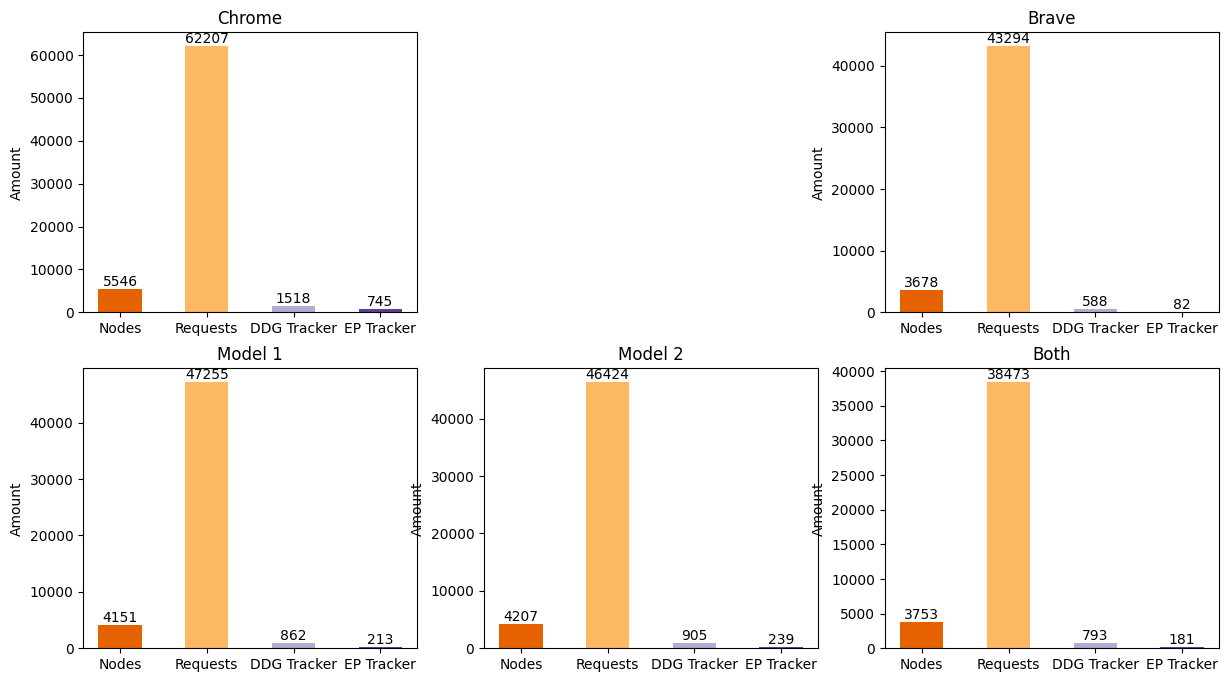
\includegraphics[width=\linewidth, keepaspectratio]{images/CrawlPlot.png}
  \caption{This figure exhibits the relevant information about each crawl of the Tranco Top 1K websites. The label \emph{DDG trackers}
    is a synonym for trackers which occur on the DuckDuckGo TPL. Moreover, \emph{EP trackers} are trackers that occur on the EasyPrivacy TPL. The \emph{nodes} show
  the number of unique domains called, and the \emph{requests} show the amount of HTTP requests performed during the crawl.}
  \label{fig:CrawlPlot}
\end{figure}
Fig-\ref{fig:CrawlPlot} showcases the relevant information gleaned from each crawl of the Tranco Top 1K websites. The bar charts in
the figure offer a comprehensive overview of the crawl data, providing insights into various aspects. The first bar in each
chart represents the number of legal entities, indicating the count of unique domains that were requested during the crawl.
The subsequent bar depicts the number of executed requests made to these legal entities. Moving forward, the following two bars
illustrate the number of trackers identified among the legal entities. The first bar reflects the trackers labeled by the DuckDuckGo\footnote{The DuckDuckGo Tracking Protection List (TPL) is a curated set of rules used by the DuckDuckGo search engine to enhance user privacy and security. It consists of domain names and patterns associated with trackers, analytics scripts, and other online tracking methods. By blocking these elements, DuckDuckGo TPL helps prevent third-party sites from collecting user data and delivering targeted ads. The list can be found here: \url{https://github.com/duckduckgo/tracker-blocklists}}
blocking list, while the second bar corresponds to the trackers labeled by the EasyPrivacy\footnote{EasyPrivacy is a well-known and widely used tracking protection list that is part of the larger EasyList project. As a comprehensive solution, EasyPrivacy is specifically designed to enhance user privacy and security while browsing the internet. It achieves this by blocking various tracking elements, such as cookies, web beacons, and tracking scripts, that are often employed by advertisers and data collection companies to monitor user behavior and deliver targeted advertisements. The list can be found here: \url{https://github.com/easylist/easylist}} blocking list.

Examining the initial crawl performed on the Chrome browser without any extensions, we discovered a total of 5,546 unique
domains. Among these domains, 1,518 were identified as trackers by the DuckDuckGo blocking list, while 745 were labeled
as trackers by the EasyPrivacy blocking list. Remarkably, the Chrome browser required a substantial number of 62,207
requests to load all 1K websites, indicating a high level of web activity.

In contrast, the Brave browser exhibited a more privacy-focused behavior during the crawl. It visited a significantly
lower number of domains, specifically 3,678, of which 588 were identified as trackers by the DuckDuckGo blocking list, and 82 were
classified as trackers by the EasyPrivacy blocking list. Furthermore, the Brave browser executed a much lower count of 43,294
requests to load all the pages. This marked difference can be attributed to the inherent advertisement and tracking blocking capabilities 
that Brave offers out of the box. To evaluate the performance of our models, we employed the Chrome browser as the baseline,
representing the level of performance our models aimed to surpass, and the Brave browser as the target, representing the desired
level of performance to be achieved.

Upon scrutinizing the performance of our two models, we made intriguing observations. Both Model 1 and Model 2 visited fewer
domains and generated fewer requests compared to the Chrome crawl. However, there were notable distinctions between the two models.
Model 1 allowed for 831 more requests than Model 2, while Model 2 visited 56 additional domains in its crawl. Comparing the bar charts
of both models with that of the Brave browser, we find striking similarities, affirming the capabilities of our models. This alignment
suggests a successful integration of the utilized technologies in achieving real-time request blocking. Moreover, both models
substantially reduced the number of identified trackers compared to the Chrome crawl. Model 1 decreased the DuckDuckGo trackers
by 656 and the EasyPrivacy trackers by 532, while Model 2 reduced the DuckDuckGo trackers by 613 and the EasyPrivacy trackers
by 506. Based on these metrics, one could argue that Model 1 outperforms Model 2 in terms of the reduced number of trackers
present in its crawl.

However, the analysis becomes more nuanced when we compare the crawls where each individual model was active. Interestingly,
both models exhibited unique blocking behaviors, resulting in the blocking of different trackers. Consequently, when both models
were simultaneously active during the crawl, the overall sum of trackers were reduced even further. Additionally, we observed that the
combined crawl yielded a lower number of requests compared to the Brave browser crawl, while the count of visited domains
approached that of the Brave crawl. This finding underscores the importance and effectiveness of having both models active
simultaneously, as it achieved the optimal performance in our real-time application.

To summarize, our analysis unequivocally demonstrates the efficacy of employing machine learning models for real-time tracking
request blocking, even approaching the performance level of the TPLs implemented in the Brave browser. 
Furthermore, it is essential to consider the effort invested in creating the Tracking Protection Lists. 
The models demonstrated here can be trained and deployed within 15 minutes, while it is challenging to keep the lists up to date. The models successfully
identify tracking requests in real-time, resulting in significantly reduced numbers of trackers, as evidenced by the plotted data.
Moreover, our web extension provides superior privacy protection compared to using the Chrome browser without any extensions, evident
in the drastic reduction in the number of requests, visited domains, and identified trackers. Consequently, we conclude that leveraging
machine learning models to block tracking web requests is a viable and promising strategy in countering web tracking, with the potential
to surpass the effectiveness of traditional TPLs when trained on robust datasets.






\subsection{Site-breakage}
One critical aspect to consider when evaluating the effectiveness of a web extension is the potential for site breakage.
Site breakage refers to any negative impact or disruption caused to websites due to the implementation of the extension's
functionalities. In our case, it pertains to the possibility of the web extension interfering with the normal functioning
and rendering of web pages.

Ensuring minimal site breakage is of utmost importance to provide users with a seamless browsing experience while benefiting
from enhanced privacy and tracking protection. In this section, we will assess the site breakage implications of our web extension.

During the development phase, we tested our extension in our day-to-day browsing usage. We are pleased to report that our web
extension demonstrated a high degree of compatibility with the majority of websites tested.
The vast majority of websites rendered correctly and maintained their full functionality when the extension was active. We
were able to navigate, interact with content, and utilize website features without experiencing any significant disruptions.

However, it is important to acknowledge that in rare cases, certain websites may exhibit minor deviations in appearance or
functionality when our web extension is active. These deviations, often occur with YouTube videos on YouTube itself or embedded 
YouTube videos on other websites. These videos do not load whenever there is an advertisement before the video starts. Moreover, 
authentication with third-party authentication services does not work. Furthermore, advertisement does not get loaded and there are empty 
spaces on the website where an advertisement should have been loaded. These deviations are typically minimal and do not significantly impact
the overall user experience or the ability to access and consume website content.

The potential for site breakage can arise due to the nature of the extension's tracking protection mechanisms. As the extension
aims to block tracking requests, there is a possibility that some websites may rely
on these components for specific functionalities or analytics. Consequently, when such elements are blocked, it can result in
minor visual inconsistencies or limited functionality. However, these occurrences are infrequent and typically do not hinder
the core usability or purpose of the websites.

In conclusion, while we acknowledge the possibility of minor site breakage in rare instances, these instances do not occur frequently 
and in that cases it is possible to disable the extension and reload the website.
\subsection{Limitations}

While our web extension provides users with valuable privacy-enhancing features and effectively blocks tracking requests,
it is crucial to recognize the limitations associated with its functionality. Understanding these limitations allows for a more
comprehensive evaluation of the extension's performance and assists in identifying areas for improvement. The following limitations
warrant attention:
\begin{enumerate}
  \item{
    \textbf{Web Crawls and Evaluation:} In order to gain a deeper understanding of the privacy-enhancing capabilities
  of the web extension, it is necessary to expand the scope of web crawls. By including a larger number of websites and
simulating user interactions with these sites, we can obtain more detailed information regarding the effectiveness of the
extension in blocking web trackers. This expanded evaluation approach would provide valuable insights into the extension's
performance across a wider range of scenarios.}
  \item{
    \textbf{User Studies and Site Breakage:} Conducting user studies is essential for evaluating the occurrence
    of site breakage when using the web extension. These studies would allow us to better understand the performance
    of the machine learning models and assess the usability of websites. By analyzing user feedback and monitoring website
    functionality during these studies, we can gain insights into potential disruptions caused by the extension and identify
    areas for improvement. This user-centric evaluation would provide valuable feedback for optimizing the extension's compatibility
    with various websites.
    }
  \item{
    \textbf{Page Loading Times:} An in-depth investigation into page loading times would provide valuable insights into the
    performance of the machine learning model. Although our initial web crawls suggest that the model performs well, it is
    important to quantify its impact on page loading times. By analyzing the time it takes for websites to load with and without
    the web extension enabled, we can assess any potential performance trade-offs and work towards optimizing the model's efficiency.
    }
\end{enumerate}

It is important to note that while our web crawls and the available data provide valuable insights. They do not offer a 
comprehensive quantitative assessment of the model's performance. Therefore, conducting more extensive web crawls, user studies,
and performance evaluations would provide a more accurate and detailed understanding of the web extension's capabilities.

By addressing these limitations, we can strive to enhance the web extension's performance, minimize site breakage, and optimize
page loading times. Regular updates, continuous evaluation, and user feedback are instrumental in refining the machine learning models
and improving the extension's overall functionality.

